\documentclass{article}
\usepackage{ctex}
\usepackage{graphicx}
\usepackage{pythonhighlight}
\graphicspath{{figure/}}

%\usepackage{listings}
%
%%%%%%%%------------------------------------------------------------------------
%%%% 日常所用宏包

%% 控制页边距
% 如果是beamer文档类, 则不用geometry
\makeatletter
\@ifclassloaded{beamer}{}{\usepackage[top=2.5cm, bottom=2.5cm, left=2.5cm, right=2.5cm]{geometry}}
\makeatother

\usepackage{amsthm}
%% 控制项目列表
\usepackage{enumerate}

%% Todo list
\usepackage{enumitem}
\newlist{todolist}{itemize}{2}
\setlist[todolist]{label=$\square$}
\usepackage{pifont}
\newcommand{\cmark}{\ding{51}}%
\newcommand{\xmark}{\ding{55}}%
\newcommand{\done}{\rlap{$\square$}{\raisebox{2pt}{\large\hspace{1pt}\cmark}}%
\hspace{-2.5pt}}
\newcommand{\wontfix}{\rlap{$\square$}{\large\hspace{1pt}\xmark}}


\usepackage{framed}

%% 多栏显示
\usepackage{multicol}

%% 算法环境
\usepackage{algorithm}  
\usepackage{algorithmic} 
\usepackage{float} 

%% 网址引用
\usepackage{url}

%% 控制矩阵行距
\renewcommand\arraystretch{1.4}

%% 粗体
\usepackage{bm}


%% hyperref宏包,生成可定位点击的超链接,并且会生成pdf书签
\makeatletter
\@ifclassloaded{beamer}{
\usepackage{hyperref}
\usepackage{ragged2e} % 对齐
}{
\usepackage[%
    pdfstartview=FitH,%
    CJKbookmarks=true,%
    bookmarks=true,%
    bookmarksnumbered=true,%
    bookmarksopen=true,%
    colorlinks=true,%
    citecolor=blue,%
    linkcolor=blue,%
    anchorcolor=green,%
    urlcolor=blue%
]{hyperref}
}
\makeatother



\makeatletter % 如果是 beamer 不需要下面两个包
\@ifclassloaded{beamer}{
\mode<presentation>
{
} 
}{
%% 控制标题
\usepackage{titlesec}
%% 控制目录
\usepackage{titletoc}
}
\makeatother

%% 控制表格样式
\usepackage{booktabs}

%% 控制字体大小
\usepackage{type1cm}

%% 首行缩进,用\noindent取消某段缩进
\usepackage{indentfirst}

%% 支持彩色文本、底色、文本框等
\usepackage{color,xcolor}

%% AMS LaTeX宏包: http://zzg34b.w3.c361.com/package/maths.htm#amssymb
\usepackage{amsmath,amssymb}
%% 多个图形并排
\usepackage{subfloat}
%%%% 基本插图方法
%% 图形宏包
\usepackage{graphicx}
\newcommand{\red}[1]{\textcolor{red}{#1}}
\newcommand{\blue}[1]{\structure{#1}}
\newcommand{\brown}[1]{\textcolor{brown}{#1}}
\newcommand{\green}[1]{\textcolor{green}{#1}}


%%%% 基本插图方法结束

%%%% pgf/tikz绘图宏包设置
\usepackage{pgf,tikz}
\usetikzlibrary{shapes,automata,snakes,backgrounds,arrows}
\usetikzlibrary{mindmap}
%% 可以直接在latex文档中使用graphviz/dot语言,
%% 也可以用dot2tex工具将dot文件转换成tex文件再include进来
%% \usepackage[shell,pgf,outputdir={docgraphs/}]{dot2texi}
%%%% pgf/tikz设置结束


\makeatletter % 如果是 beamer 不需要下面两个包
\@ifclassloaded{beamer}{

}{
%%%% fancyhdr设置页眉页脚
%% 页眉页脚宏包
\usepackage{fancyhdr}
%% 页眉页脚风格
\pagestyle{plain}
}

%% 有时会出现\headheight too small的warning
\setlength{\headheight}{15pt}

%% 清空当前页眉页脚的默认设置
%\fancyhf{}
%%%% fancyhdr设置结束


\usepackage{listings}
%% 设置listings宏包的一些全局样式
%% 参考http://hi.baidu.com/shawpinlee/blog/item/9ec431cbae28e41cbe09e6e4.html
\lstset{
showstringspaces=false,              %% 设定是否显示代码之间的空格符号
numbers=left,                        %% 在左边显示行号
numberstyle=\tiny,                   %% 设定行号字体的大小
basicstyle=\scriptsize,                    %% 设定字体大小\tiny, \small, \Large等等
keywordstyle=\color{blue!70}, commentstyle=\color{red!50!green!50!blue!50},
                                     %% 关键字高亮
frame=shadowbox,                     %% 给代码加框
rulesepcolor=\color{red!20!green!20!blue!20},
escapechar=`,                        %% 中文逃逸字符,用于中英混排
xleftmargin=2em,xrightmargin=2em, aboveskip=1em,
breaklines,                          %% 这条命令可以让LaTeX自动将长的代码行换行排版
extendedchars=false                  %% 这一条命令可以解决代码跨页时,章节标题,页眉等汉字不显示的问题
}

\usepackage{minted}
\renewcommand{\listingscaption}{Python code} \newminted{python}{
    escapeinside=||,
    mathescape=true,
    numbersep=5pt,
    linenos=true,
    autogobble,
    framesep=3mm} 
%%%% listings宏包设置结束


%%%% 附录设置
\makeatletter % 对 beamer 要重新设置
\@ifclassloaded{beamer}{

}{
\usepackage[title,titletoc,header]{appendix}
}
\makeatother
%%%% 附录设置结束





%% 设定行距
\linespread{1}

%% 粗体的小写字母代表向量或向量函数
\newcommand{\bfa}{{\boldsymbol a}}
\newcommand{\bfb}{{\boldsymbol b}}
\newcommand{\bfc}{{\boldsymbol c}}
\newcommand{\bfd}{{\boldsymbol d}}
\newcommand{\bfe}{{\boldsymbol e}}
\newcommand{\bff}{{\boldsymbol f}}
\newcommand{\bfg}{{\boldsymbol g}}
\newcommand{\bfh}{{\boldsymbol h}}
\newcommand{\bfi}{{\boldsymbol i}}
\newcommand{\bfj}{{\boldsymbol j}}
\newcommand{\bfk}{{\boldsymbol k}}
\newcommand{\bfl}{{\boldsymbol l}}
\newcommand{\bfm}{{\boldsymbol m}}
\newcommand{\bfn}{{\boldsymbol n}}
\newcommand{\bfo}{{\boldsymbol o}}
\newcommand{\bfp}{{\boldsymbol p}}
\newcommand{\bfq}{{\boldsymbol q}}
\newcommand{\bfr}{{\boldsymbol r}}
\newcommand{\bfs}{{\boldsymbol s}}
\newcommand{\bft}{{\boldsymbol t}}
\newcommand{\bfu}{{\boldsymbol u}}
\newcommand{\bfv}{{\boldsymbol v}}
\newcommand{\bfw}{{\boldsymbol w}}
\newcommand{\bfx}{{\boldsymbol x}}
\newcommand{\bfy}{{\boldsymbol y}}
\newcommand{\bfz}{{\boldsymbol z}}

% 线性变换空间
\newcommand{\mca}{{\mathcal a}}
\newcommand{\mcb}{{\mathcal b}}
\newcommand{\mcc}{{\mathcal c}}
\newcommand{\mcd}{{\mathcal d}}
\newcommand{\mce}{{\mathcal e}}
\newcommand{\mcf}{{\mathcal f}}
\newcommand{\mcg}{{\mathcal g}}
\newcommand{\mch}{{\mathcal h}}
\newcommand{\mci}{{\mathcal i}}
\newcommand{\mcj}{{\mathcal j}}
\newcommand{\mck}{{\mathcal k}}
\newcommand{\mcl}{{\mathcal l}}
\newcommand{\mcm}{{\mathcal m}}
\newcommand{\mcn}{{\mathcal n}}
\newcommand{\mco}{{\mathcal o}}
\newcommand{\mcp}{{\mathcal p}}
\newcommand{\mcq}{{\mathcal q}}
\newcommand{\mcr}{{\mathcal r}}
\newcommand{\mcs}{{\mathcal s}}
\newcommand{\mct}{{\mathcal t}}
\newcommand{\mcu}{{\mathcal u}}
\newcommand{\mcv}{{\mathcal v}}
\newcommand{\mcw}{{\mathcal w}}
\newcommand{\mcx}{{\mathcal x}}
\newcommand{\mcy}{{\mathcal y}}
\newcommand{\mcz}{{\mathcal z}}

\newcommand{\mra}{{\mathrm a}}
\newcommand{\mrb}{{\mathrm b}}
\newcommand{\mrc}{{\mathrm c}}
\newcommand{\mrd}{{\mathrm d}}
\newcommand{\mre}{{\mathrm e}}
\newcommand{\mrf}{{\mathrm f}}
\newcommand{\mrg}{{\mathrm g}}
\newcommand{\mrh}{{\mathrm h}}
\newcommand{\mri}{{\mathrm i}}
\newcommand{\mrj}{{\mathrm j}}
\newcommand{\mrk}{{\mathrm k}}
\newcommand{\mrl}{{\mathrm l}}
\newcommand{\mrm}{{\mathrm m}}
\newcommand{\mrn}{{\mathrm n}}
\newcommand{\mro}{{\mathrm o}}
\newcommand{\mrp}{{\mathrm p}}
\newcommand{\mrq}{{\mathrm q}}
\newcommand{\mrr}{{\mathrm r}}
\newcommand{\mrs}{{\mathrm s}}
\newcommand{\mrt}{{\mathrm t}}
\newcommand{\mru}{{\mathrm u}}
\newcommand{\mrv}{{\mathrm v}}
\newcommand{\mrw}{{\mathrm w}}
\newcommand{\mrx}{{\mathrm x}}
\newcommand{\mry}{{\mathrm y}}
\newcommand{\mrz}{{\mathrm z}}

%% 粗体的大写字母一般表示矩阵和张量
\newcommand{\bfA}{{\boldsymbol A}}
\newcommand{\bfB}{{\boldsymbol B}}
\newcommand{\bfC}{{\boldsymbol C}}
\newcommand{\bfD}{{\boldsymbol D}}
\newcommand{\bfE}{{\boldsymbol E}}
\newcommand{\bfF}{{\boldsymbol F}}
\newcommand{\bfG}{{\boldsymbol G}}
\newcommand{\bfH}{{\boldsymbol H}}
\newcommand{\bfI}{{\boldsymbol I}}
\newcommand{\bfJ}{{\boldsymbol J}}
\newcommand{\bfK}{{\boldsymbol K}}
\newcommand{\bfL}{{\boldsymbol L}}
\newcommand{\bfM}{{\boldsymbol M}}
\newcommand{\bfN}{{\boldsymbol N}}
\newcommand{\bfO}{{\boldsymbol O}}
\newcommand{\bfP}{{\boldsymbol P}}
\newcommand{\bfQ}{{\boldsymbol Q}}
\newcommand{\bfR}{{\boldsymbol R}}
\newcommand{\bfS}{{\boldsymbol S}}
\newcommand{\bfT}{{\boldsymbol T}}
\newcommand{\bfU}{{\boldsymbol U}}
\newcommand{\bfV}{{\boldsymbol V}}
\newcommand{\bfW}{{\boldsymbol W}}
\newcommand{\bfX}{{\boldsymbol X}}
\newcommand{\bfY}{{\boldsymbol Y}}
\newcommand{\bfZ}{{\boldsymbol Z}}

%% 花体大写字母
\newcommand{\mcA}{{\mathcal A}}
\newcommand{\mcB}{{\mathcal B}}
\newcommand{\mcC}{{\mathcal C}}
\newcommand{\mcD}{{\mathcal D}}
\newcommand{\mcE}{{\mathcal E}}
\newcommand{\mcF}{{\mathcal F}}
\newcommand{\mcG}{{\mathcal G}}
\newcommand{\mcH}{{\mathcal H}}
\newcommand{\mcI}{{\mathcal I}}
\newcommand{\mcJ}{{\mathcal J}}
\newcommand{\mcK}{{\mathcal K}}
\newcommand{\mcL}{{\mathcal L}}
\newcommand{\mcM}{{\mathcal M}}
\newcommand{\mcN}{{\mathcal N}}
\newcommand{\mcO}{{\mathcal O}}
\newcommand{\mcP}{{\mathcal P}}
\newcommand{\mcQ}{{\mathcal Q}}
\newcommand{\mcR}{{\mathcal R}}
\newcommand{\mcS}{{\mathcal S}}
\newcommand{\mcT}{{\mathcal T}}
\newcommand{\mcU}{{\mathcal U}}
\newcommand{\mcV}{{\mathcal V}}
\newcommand{\mcW}{{\mathcal W}}
\newcommand{\mcX}{{\mathcal X}}
\newcommand{\mcY}{{\mathcal Y}}
\newcommand{\mcZ}{{\mathcal Z}}

%% 空心大写字母
\newcommand{\mbA}{{\mathbb A}}
\newcommand{\mbB}{{\mathbb B}}
\newcommand{\mbC}{{\mathbb C}}
\newcommand{\mbD}{{\mathbb D}}
\newcommand{\mbE}{{\mathbb E}}
\newcommand{\mbF}{{\mathbb F}}
\newcommand{\mbG}{{\mathbb G}}
\newcommand{\mbH}{{\mathbb H}}
\newcommand{\mbI}{{\mathbb I}}
\newcommand{\mbJ}{{\mathbb J}}
\newcommand{\mbK}{{\mathbb K}}
\newcommand{\mbL}{{\mathbb L}}
\newcommand{\mbM}{{\mathbb M}}
\newcommand{\mbN}{{\mathbb N}}
\newcommand{\mbO}{{\mathbb O}}
\newcommand{\mbP}{{\mathbb P}}
\newcommand{\mbQ}{{\mathbb Q}}
\newcommand{\mbR}{{\mathbb R}}
\newcommand{\mbS}{{\mathbb S}}
\newcommand{\mbT}{{\mathbb T}}
\newcommand{\mbU}{{\mathbb U}}
\newcommand{\mbV}{{\mathbb V}}
\newcommand{\mbW}{{\mathbb W}}
\newcommand{\mbX}{{\mathbb X}}
\newcommand{\mbY}{{\mathbb Y}}
\newcommand{\mbZ}{{\mathbb Z}}

\newcommand{\mrA}{{\mathrm A}}
\newcommand{\mrB}{{\mathrm B}}
\newcommand{\mrC}{{\mathrm C}}
\newcommand{\mrD}{{\mathrm D}}
\newcommand{\mrE}{{\mathrm E}}
\newcommand{\mrF}{{\mathrm F}}
\newcommand{\mrG}{{\mathrm G}}
\newcommand{\mrH}{{\mathrm H}}
\newcommand{\mrI}{{\mathrm I}}
\newcommand{\mrJ}{{\mathrm J}}
\newcommand{\mrK}{{\mathrm K}}
\newcommand{\mrL}{{\mathrm L}}
\newcommand{\mrM}{{\mathrm M}}
\newcommand{\mrN}{{\mathrm N}}
\newcommand{\mrO}{{\mathrm O}}
\newcommand{\mrP}{{\mathrm P}}
\newcommand{\mrQ}{{\mathrm Q}}
\newcommand{\mrR}{{\mathrm R}}
\newcommand{\mrS}{{\mathrm S}}
\newcommand{\mrT}{{\mathrm T}}
\newcommand{\mrU}{{\mathrm U}}
\newcommand{\mrV}{{\mathrm V}}
\newcommand{\mrW}{{\mathrm W}}
\newcommand{\mrX}{{\mathrm X}}
\newcommand{\mrY}{{\mathrm Y}}
\newcommand{\mrZ}{{\mathrm Z}}


% 粗体的 Greek 字母
\newcommand{\balpha}{{\bm \alpha}}
\newcommand{\bbeta}{{\bm \beta}}
\newcommand{\bgamma}{{\bm \gamma}}
\newcommand{\bdelta}{{\bm \delta}}
\newcommand{\bepsilon}{{\bm \epsilon}}
\newcommand{\bvarepsilon}{{\bm \varepsilon}}
\newcommand{\bzeta}{{\bm \zeta}}
\newcommand{\bfeta}{{\bm \eta}}
\newcommand{\btheta}{{\bm \theta}}
\newcommand{\biota}{{\bm \iota}}
\newcommand{\bkappa}{{\bm \kappa}}
\newcommand{\blambda}{{\bm \lambda}}
\newcommand{\bmu}{{\bm \mu}}
\newcommand{\bnu}{{\bm \nu}}
\newcommand{\bxi}{{\bm \xi}}
\newcommand{\bomicron}{{\bm \omicron}}
\newcommand{\bpi}{{\bm \pi}}
\newcommand{\brho}{{\bm \rho}}
\newcommand{\bsigma}{{\bm \sigma}}
\newcommand{\btau}{{\bm \tau}}
\newcommand{\bupsilon}{{\bm \upsilon}}
\newcommand{\bphi}{{\bm \phi}}
\newcommand{\bchi}{{\bm \chi}}
\newcommand{\bpsi}{{\bm \psi}}

\newcommand{\bAlpha}{{\bm \Alpha}}
\newcommand{\bBeta}{{\bm \Beta}}
\newcommand{\bGamma}{{\bm \Gamma}}
\newcommand{\bDelta}{{\bm \Delta}}
\newcommand{\bEpsilon}{{\bm \Psilon}}
\newcommand{\bVarepsilon}{{\bm \Varepsilon}}
\newcommand{\bZeta}{{\bm \Zeta}}
\newcommand{\bEta}{{\bm \Eta}}
\newcommand{\bTheta}{{\bm \Theta}}
\newcommand{\bIota}{{\bm \Iota}}
\newcommand{\bKappa}{{\bm \Kappa}}
\newcommand{\bLambda}{{\bm \Lambda}}
\newcommand{\bMu}{{\bm \Mu}}
\newcommand{\bNu}{{\bm \Nu}}
\newcommand{\bXi}{{\bm \Xi}}
\newcommand{\bOmicron}{{\bm \Omicron}}
\newcommand{\bPi}{{\bm \Pi}}
\newcommand{\bRho}{{\bm \Rho}}
\newcommand{\bSigma}{{\bm \Sigma}}
\newcommand{\bTau}{{\bm \Tau}}
\newcommand{\bUpsilon}{{\bm \Upsilon}}
\newcommand{\bPhi}{{\bm \Phi}}
\newcommand{\bChi}{{\bm \Chi}}
\newcommand{\bPsi}{{\bm \Psi}}

\newcommand{\rmd}{\,\mathrm d}
\newcommand{\bfzero}{\mathbf 0}

%% 算子
\newcommand{\ospan}{\operatorname{span}}
\newcommand{\odiv}{\operatorname{div}}
\newcommand{\otr}{\operatorname{tr}}
\newcommand{\ograd}{\operatorname{grad}}
\newcommand{\orot}{\operatorname{rot}}
\newcommand{\ocurl}{\operatorname{curl}}
\newcommand{\odist}{\operatorname{dist}}
\newcommand{\osign}{\operatorname{sign}}
\newcommand{\odiag}{\operatorname{diag}}

\newcommand{\od}{\text{div}}
\newcommand{\os}{\text{span}}
\newcommand{\ot}{\text{tr}}
\newcommand{\norm}[1]{||#1||}
\newcommand{\dof}{\text{dof}}

%%%% 个性设置结束
%%%%%%%%------------------------------------------------------------------------


%%%%%%%%------------------------------------------------------------------------
%%%% bibtex设置

%% 设定参考文献显示风格
% 下面是几种常见的样式
% * plain: 按字母的顺序排列,比较次序为作者、年度和标题
% * unsrt: 样式同plain,只是按照引用的先后排序
% * alpha: 用作者名首字母+年份后两位作标号,以字母顺序排序
% * abbrv: 类似plain,将月份全拼改为缩写,更显紧凑
% * apalike: 美国心理学学会期刊样式, 引用样式 [Tailper and Zang, 2006]

%\makeatletter
%\@ifclassloaded{beamer}{
%\bibliographystyle{apalike}
%}{
%\bibliographystyle{abbrv}
%}
%\makeatother


%%%% bibtex设置结束
%%%%%%%%------------------------------------------------------------------------

%%%%%%%%%------------------------------------------------------------------------
%%%% xeCJK相关宏包

\usepackage{xltxtra,fontspec,xunicode}
\usepackage[slantfont, boldfont]{xeCJK} 

\setlength{\parindent}{2em}%中文缩进两个汉字位

%% 针对中文进行断行
\XeTeXlinebreaklocale "zh"             

%% 给予TeX断行一定自由度
\XeTeXlinebreakskip = 0pt plus 1pt minus 0.1pt

%%%% xeCJK设置结束                                       
%%%%%%%%------------------------------------------------------------------------

%%%%%%%%------------------------------------------------------------------------
%%%% xeCJK字体设置

%% 设置中文标点样式,支持quanjiao、banjiao、kaiming等多种方式
\punctstyle{kaiming}                                        
                                                     
%% 设置缺省中文字体
%\setCJKmainfont[BoldFont={Adobe Heiti Std}, ItalicFont={Adobe Kaiti Std}]{Adobe Song Std}   
\setCJKmainfont{Adobe Kaiti Std}
%% 设置中文无衬线字体
%\setCJKsansfont[BoldFont={Adobe Heiti Std}]{Adobe Kaiti Std}  
%% 设置等宽字体
%\setCJKmonofont{Adobe Heiti Std}                            

%% 英文衬线字体
\setmainfont{DejaVu Serif}                                  
%% 英文等宽字体
\setmonofont{DejaVu Sans Mono}                              
%% 英文无衬线字体
\setsansfont{DejaVu Sans}                                   

%% 定义新字体
\setCJKfamilyfont{song}{Adobe Song Std}                     
\setCJKfamilyfont{kai}{Adobe Kaiti Std}
\setCJKfamilyfont{hei}{Adobe Heiti Std}
\setCJKfamilyfont{fangsong}{Adobe Fangsong Std}
\setCJKfamilyfont{lisu}{LiSu}
\setCJKfamilyfont{youyuan}{YouYuan}

%% 自定义宋体
\newcommand{\song}{\CJKfamily{song}}                       
%% 自定义楷体
\newcommand{\kai}{\CJKfamily{kai}}                         
%% 自定义黑体
\newcommand{\hei}{\CJKfamily{hei}}                         
%% 自定义仿宋体
\newcommand{\fangsong}{\CJKfamily{fangsong}}               
%% 自定义隶书
\newcommand{\lisu}{\CJKfamily{lisu}}                       
%% 自定义幼圆
\newcommand{\youyuan}{\CJKfamily{youyuan}}                 

%%%% xeCJK字体设置结束
%%%%%%%%------------------------------------------------------------------------

%%%%%%%%------------------------------------------------------------------------
%%%% 一些关于中文文档的重定义
\newcommand{\chntoday}{\number\year\,年\,\number\month\,月\,\number\day\,日}
%% 数学公式定理的重定义

%% 中文破折号,据说来自清华模板
\newcommand{\pozhehao}{\kern0.3ex\rule[0.8ex]{2em}{0.1ex}\kern0.3ex}

\makeatletter %
\@ifclassloaded{beamer}{

}{
\newtheorem{example}{例}                                   
\newtheorem{theorem}{定理}[section]                         
\newtheorem{definition}{定义}
\newtheorem{axiom}{公理}
\newtheorem{property}{性质}
\newtheorem{proposition}{命题}
\newtheorem{lemma}{引理}
\newtheorem{corollary}{推论}
\newtheorem{remark}{注解}
\newtheorem{condition}{条件}
\newtheorem{conclusion}{结论}
\newtheorem{assumption}{假设}
}
\makeatother

\makeatletter %
\@ifclassloaded{beamer}{

}{
%% 章节等名称重定义
\renewcommand{\contentsname}{目录}     
\renewcommand{\indexname}{索引}
\renewcommand{\listfigurename}{插图目录}
\renewcommand{\listtablename}{表格目录}
\renewcommand{\appendixname}{附录}
\renewcommand{\appendixpagename}{附录}
\renewcommand{\appendixtocname}{附录}
\@ifclassloaded{book}{

}{
\renewcommand{\abstractname}{摘要}
}
}
\makeatother

\renewcommand{\figurename}{图}
\renewcommand{\tablename}{表}

\makeatletter
\@ifclassloaded{book}{
\renewcommand{\bibname}{参考文献}
}{
\renewcommand{\refname}{参考文献} 
}
\makeatother

\floatname{algorithm}{算法}
\renewcommand{\algorithmicrequire}{\textbf{输入:}}
\renewcommand{\algorithmicensure}{\textbf{输出:}}

\renewcommand{\today}{\number\year 年 \number\month 月 \number\day 日}

%%%% 中文重定义结束
%%%%%%%%------------------------------------------------------------------------

%\usepackage{xcolor}

%\lstset{
%	basicstyle          =   \sffamily,          % 基本代码风格
%	keywordstyle        =   \bfseries,          % 关键字风格
%	commentstyle        =   \rmfamily\itshape,  % 注释的风格,斜体
%	stringstyle         =   \ttfamily,  % 字符串风格
%	flexiblecolumns,                % 别问为什么,加上这个
%	numbers             =   left,   % 行号的位置在左边
%	showspaces          =   false,  % 是否显示空格,显示了有点乱,所以不现实了
%	numberstyle         =   \zihao{-5}\ttfamily,    % 行号的样式,小五号,tt等宽字体
%	showstringspaces    =   false,
%	captionpos          =   t,      % 这段代码的名字所呈现的位置,t指的是top上面
%	frame               =   lrtb,   % 显示边框
%}
%
%\lstdefinestyle{Python}{
%	language        =   Python, % 语言选Python
%	basicstyle      =   \zihao{-5}\ttfamily,
%	numberstyle     =   \zihao{-5}\ttfamily,
%	keywordstyle    =   \color{blue},
%	keywordstyle    =   [2] \color{teal},
%	stringstyle     =   \color{magenta},
%	commentstyle    =   \color{red}\ttfamily,
%	breaklines      =   true,   % 自动换行,建议不要写太长的行
%	columns         =   fixed,  % 如果不加这一句,字间距就不固定,很丑,必须加
%	basewidth       =   0.5em,
%}

%\usepackage{xcolor}
%\lstset{
%	numbers=left, 
%	numberstyle= \tiny, 
%	keywordstyle= \color{ blue!70},
%	commentstyle= \color{red!50!green!50!blue!50}, 
%	frame=shadowbox, % 阴影效果
%	rulesepcolor= \color{ red!20!green!20!blue!20} ,
%	escapeinside=``, % 英文分号中可写入中文
%	xleftmargin=2em,xrightmargin=2em, aboveskip=1em,
%	framexleftmargin=2em
%}




\title{周报}
\author{Shixiang Yan}
\date{\today}

\begin{document}
	\maketitle
	\tableofcontents
	\section{关于卫星天线仿真}
	我认为应该先从软件着手,对于STK我发现了有Matlab,C,C++,C\#,Java的接口。综合考虑开发难度,开发工作量以及业务需求,Matlab是最可靠的接口开发工具。本周我学习了MATLAB的相关知识,对其工作流程有了大致的了解。
	
	对于总体设计,我的想法是先在一台计算机上把所需功能跑出来,然后再考虑分布式到多台电脑上并行计算。下周我准备利用Matlab开发一个简单的可以与STK进行交互可视化程序。
	
	以下是我近期对Matlab学习所书写的部分代码:
	\subsection{结构}
	\subsubsection{顺序}
	\subsubsection{选择}
	\begin{python}
		%switch
		input_num=1;
		switch input_num
		case -1
		disp('negative 1');
		case 0
		disp('zero');
		case 1
		disp('positive 1');
		otherwise
		disp('other value');
		end        
	\end{python}
	\subsubsection{循环}
	\begin{python}
		%while循环
		n=1;
		while prod(1:n)<1e100 %Á¬³Ë
		n=n+1;
		end
		disp(n)
		%for循环
		for n=1:10
		a(n)=2^n;
		end
		disp(a)
		%%
		tic
		for ii=1:2000
		for jj=1:2000
		A(ii,jj)=ii+jj;
		end
		end
		toc
		%%
		tic
		A=zeros(2000,2000);
		for ii=1:size(A,1)
		for jj=1:size(A,2)
		A(ii,jj)=ii+jj;
		end
		end
		toc
	\end{python}
	\subsection{matlab声明函数}
	\begin{python}
		function result = fun2( a,b )
		%UNTITLED2 此处显示有关此函数的摘要
		%   此处显示详细说明
		s=0;
		for i=a:b
		s=s+i;
		end
		result=s;
		end
	\end{python}
	\subsection{画图}
	\subsubsection{正弦曲线}
	\begin{python}
		hold on
		plot(cos(0:pi/20:pi*2));
		plot(sin(0:pi/20:pi*2),'xg:');
		hold off
	\end{python}

	如图\ref{fig1}:
	
	\begin{figure}[h]
		\centering
		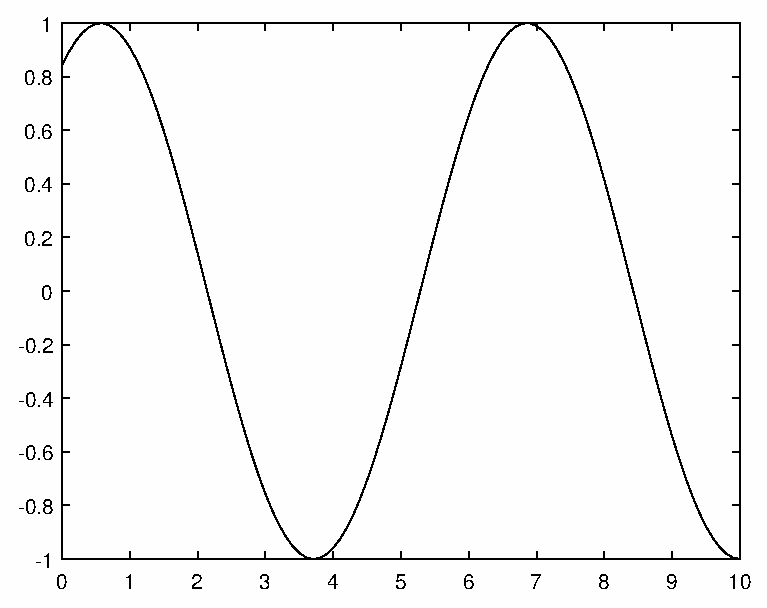
\includegraphics{plot1.ps}
		\caption{正弦曲线}\label{fig1}
	\end{figure}
	\section{关于Pytorch模块的学习}
	\subsection{numpy和pytorch}
	以下是近期我对Pytorch进行学习所书写的部分代码。
	\begin{python}
		#官网说明书:https://pytorch.org/docs/stable/torch.html
		import torch
		import numpy as np
		
		np_data = np.arange(6).reshape((2, 3))
		torch_data = torch.from_numpy(np_data)
		tensor2array = torch_data.numpy()
		print(
		'\nnumpy array:', np_data,          # [[0 1 2], [3 4 5]]
		'\ntorch tensor:', torch_data,      #  0  1  2 \n 3  4  5    [torch.LongTensor of size 2x3]
		'\ntensor to array:', tensor2array, # [[0 1 2], [3 4 5]]
		)
		
		# abs 绝对值计算
		data = [-1, -2, 1, 2]
		tensor = torch.FloatTensor(data)  # 转换成32位浮点 tensor
		print(
		'\nabs',
		'\nnumpy: ', np.abs(data),          # [1 2 1 2]
		'\ntorch: ', torch.abs(tensor)      # [1 2 1 2]
		)
		
		# sin   三角函数 sin
		print(
		'\nsin',
		'\nnumpy: ', np.sin(data),      # [-0.84147098 -0.90929743  0.84147098  0.90929743]
		'\ntorch: ', torch.sin(tensor)  # [-0.8415 -0.9093  0.8415  0.9093]
		)
		
		# mean  均值
		print(
		'\nmean',
		'\nnumpy: ', np.mean(data),         # 0.0
		'\ntorch: ', torch.mean(tensor)     # 0.0
		)
		
		# matrix multiplication 矩阵点乘
		data = [[1,2], [3,4]]
		tensor = torch.FloatTensor(data)  # 转换成32位浮点 tensor
		# correct method
		print(
		'\nmatrix multiplication (matmul)',
		'\nnumpy: ', np.matmul(data, data),     # [[7, 10], [15, 22]]
		'\ntorch: ', torch.mm(tensor, tensor)   # [[7, 10], [15, 22]]
		)
		
		# !!!!  下面是错误的方法 !!!!
		data = np.array(data)
		print(
		'\nmatrix multiplication (dot)',
		'\nnumpy: ', data.dot(data),        # [[7, 10], [15, 22]] 在numpy 中可行
		# '\ntorch: ', tensor.dot(tensor)     # torch 会转换成 [1,2,3,4].dot([1,2,3,4) = 30.0
		#'tensor.dot(tensor)',      torch 会转换成 [1,2,3,4].dot([1,2,3,4) = 30.0
		# 变为
		# '\ntorch:',torch.dot(tensor.dot(tensor))
		)
		\subsection{有关variable}
		\begin{python}
			import torch
			from torch.autograd import Variable # torch 中 Variable 模块
			
			# 先生鸡蛋
			tensor = torch.FloatTensor([[1,2],[3,4]])
			# 把鸡蛋放到篮子里, requires_grad是参不参与误差反向传播, 要不要计算梯度
			variable = Variable(tensor, requires_grad=True)
			
			print(tensor)
			"""
			1  2
			3  4
			[torch.FloatTensor of size 2x2]
			"""
			
			print(variable)
			"""
			Variable containing:
			1  2
			3  4
			[torch.FloatTensor of size 2x2]
			"""
			
			t_out = torch.mean(tensor*tensor)       # x^2
			v_out = torch.mean(variable*variable)   # x^2
			print(t_out)
			print(v_out)    # 7.5
			
			v_out.backward()    # 模拟 v_out 的误差反向传递,反向传递求梯度。
			
			# 下面两步看不懂没关系, 只要知道 Variable 是计算图的一部分, 可以用来传递误差就好.
			# v_out = 1/4 * sum(variable*variable) 这是计算图中的 v_out 计算步骤
			# 针对于 v_out 的梯度就是, d(v_out)/d(variable) = 1/4*2*variable = variable/2
			
			print(variable.grad)    # 初始 Variable 的梯度
			'''
			0.5000  1.0000
			1.5000  2.0000
			'''
			
			print(variable)     #  Variable 形式
			"""
			Variable containing:
			1  2
			3  4
			[torch.FloatTensor of size 2x2]
			"""
			
			print(variable.data)    # tensor 形式
			"""
			1  2
			3  4
			[torch.FloatTensor of size 2x2]
			"""
			
			print(variable.data.numpy())    # numpy 形式
			"""
			[[ 1.  2.]
			[ 3.  4.]]
			"""
		\end{python}
	\subsection{激活函数}
	\begin{python}
		import torch
		import torch.nn.functional as F     # 激励函数都在这
		from torch.autograd import Variable
		
		# 做一些假数据来观看图像
		x = torch.linspace(-5, 5, 200)  # x data (tensor), shape=(100, 1)
		x = Variable(x)
		
		x_np = x.data.numpy()   # 换成 numpy array, 出图时用,张量转numpy
		
		# 几种常用的 激励函数
		y_relu = torch.relu(x).data.numpy()
		y_sigmoid = torch.sigmoid(x).data.numpy()
		y_tanh = torch.tanh(x).data.numpy()
		y_softplus = F.softplus(x).data.numpy()
		# y_softmax = F.softmax(x)  softmax 比较特殊, 不能直接显示, 不过他是关于概率的, 用于分类
		
		import matplotlib.pyplot as plt  # python 的可视化模块, 我有教程 (https://morvanzhou.github.io/tutorials/data-manipulation/plt/)
		
		plt.figure(1, figsize=(8, 6))
		plt.subplot(221)
		plt.plot(x_np, y_relu, c='red', label='relu')
		plt.ylim((-1, 5))
		plt.legend(loc='best')
		
		plt.subplot(222)
		plt.plot(x_np, y_sigmoid, c='red', label='sigmoid')
		plt.ylim((-0.2, 1.2))
		plt.legend(loc='best')
		
		plt.subplot(223)
		plt.plot(x_np, y_tanh, c='red', label='tanh')
		plt.ylim((-1.2, 1.2))
		plt.legend(loc='best')
		
		plt.subplot(224)
		plt.plot(x_np, y_softplus, c='red', label='softplus')
		plt.ylim((-0.2, 6))
		plt.legend(loc='best')
		
		plt.show()
	\end{python}
	\subsection{Regressin}
	\begin{python}
		import torch
		import matplotlib.pyplot as plt
		
		x = torch.unsqueeze(torch.linspace(-1, 1, 100), dim=1)  \# x data (tensor), shape=(100, 1),数据维度进行扩充
		y = x.pow(2) + 0.2*torch.rand(x.size())                 \# noisy y data (tensor), shape=(100, 1),生成与x形状相同的y
		
		\# 画图
		plt.scatter(x.data.numpy(), y.data.numpy())
		plt.show()
		
		class Net(torch.nn.Module):  \# 继承 torch 的 Module
		def \_\_init\_\_(self, n\_feature, n\_hidden, n\_output):
		super(Net, self).\_\_init\_\_()     \# 继承 \_\_init\_\_ 功能
		\# 定义每层用什么样的形式
		self.hidden = torch.nn.Linear(n\_feature, n\_hidden)   \# 隐藏层线性输出,nn.Linear表示y=wx+b
		self.predict = torch.nn.Linear(n\_hidden, n\_output)   \# 输出层线性输出
		
		def forward(self, x):   \# 这同时也是 Module 中的 forward 功能
		\# 正向传播输入值, 神经网络分析出输出值
		x = torch.relu(self.hidden(x))      \# 激励函数(隐藏层的线性值)
		x = self.predict(x)             \# 输出值
		return x
		
		net = Net(n\_feature=1, n\_hidden=10, n\_output=1)
		
		print(net)  \# net 的结构
		"""
		Net (
		(hidden): Linear (1 -> 10)
		(predict): Linear (10 -> 1)
		)
		"""
		
		\# optimizer 是训练的工具
		optimizer = torch.optim.SGD(net.parameters(), lr=0.2)  \# 传入 net 的所有参数, 学习率
		loss\_func = torch.nn.MSELoss()      \# 预测值和真实值的误差计算公式 (均方差)
		
		for t in range(100):
		prediction = net(x)     \# 喂给 net 训练数据 x, 输出预测值
		
		loss = loss\_func(prediction, y)     \# 计算两者的误差
		
		optimizer.zero\_grad()   \# 清空上一步的残余更新参数值
		loss.backward()         \# 误差反向传播, 计算参数更新值
		optimizer.step()        \# 将参数更新值施加到 net 的 parameters 上
		
		\# import matplotlib.pyplot as plt
		
		plt.ion()   \# 画图
		plt.show()
		
		for t in range(50):
		
		prediction = net(x)  \# 喂给 net 训练数据 x, 输出预测值
		
		loss = loss\_func(prediction, y)  \# 计算两者的误差
		
		optimizer.zero\_grad()  \# 清空上一步的残余更新参数值
		loss.backward()
		optimizer.step()
		
		\# 接着上面来
		if t \% 10 == 0:
		\# plot and show learning process
		plt.cla()
		plt.scatter(x.data.numpy(), y.data.numpy())
		plt.plot(x.data.numpy(), prediction.data.numpy(), 'r-', lw=5)
		plt.text(0.5, 0, 'Loss=\%.4f' \% loss.data.numpy(), fontdict=\{'size': 20, 'color':  'red'\})
		plt.pause(0.1)
	\end{python}
	\subsection{classification}
		\begin{python}
			import torch
			import matplotlib.pyplot as plt
			
			# 假数据
			n_data = torch.ones(100, 2)         # 数据的基本形态
			
			x0 = torch.normal(2*n_data, 1)      # 类型0 x data (tensor), shape=(100, 2)
			help(torch.normal)
			print(x0)
			y0 = torch.zeros(100)               # 类型0 y data (tensor), shape=(100, )
			x1 = torch.normal(-2*n_data, 1)     # 类型1 x data (tensor), shape=(100, 1)
			y1 = torch.ones(100)                # 类型1 y data (tensor), shape=(100, )
			
			# 注意 x, y 数据的数据形式是一定要像下面一样 (torch.cat 是在合并数据)
			x = torch.cat((x0, x1), 0).type(torch.FloatTensor)  # FloatTensor = 32-bit floating
			y = torch.cat((y0, y1), ).type(torch.LongTensor)    # LongTensor = 64-bit integer
			
			plt.scatter(x.data.numpy()[:, 0], x.data.numpy()[:, 1], c=y.data.numpy(), s=100, lw=0, cmap='RdYlGn')
			plt.show()
			
			# 画图
			# plt.scatter(x.data.numpy(), y.data.numpy())
			# plt.show()
			
			import torch
			import torch.nn.functional as F     # 激励函数都在这
			
			#搭建正向传递网络方式一:
			class Net(torch.nn.Module):     # 继承 torch 的 Module
			def __init__(self, n_feature, n_hidden, n_output):
			super(Net, self).__init__()     # 继承 __init__ 功能
			self.hidden = torch.nn.Linear(n_feature, n_hidden)   # 隐藏层线性输出
			self.out = torch.nn.Linear(n_hidden, n_output)       # 输出层线性输出
			
			def forward(self, x):
			# 正向传播输入值, 神经网络分析出输出值
			x = F.relu(self.hidden(x))      # 激励函数(隐藏层的线性值)
			x = self.out(x)                 # 输出值, 但是这个不是预测值, 预测值还需要再另外计算
			return x
			
			net = Net(n_feature=2, n_hidden=10, n_output=2) # 几个类别就几个 output
			
			print(net)  # net 的结构
			"""
			Net (
			(hidden): Linear (2 -> 10)
			(out): Linear (10 -> 2)
			)
			"""
			# #搭建正向传递方式二:
			# net2 = torch.nn.Sequential(
			#     torch.nn.Linear(2, 10),
			#     torch.nn.ReLU(),
			#     torch.nn.Linear(10, 2)
			# )
			
			
			# optimizer 是训练的工具
			optimizer = torch.optim.SGD(net.parameters(), lr=0.02)  # 传入 net 的所有参数, 学习率
			# 算误差的时候, 注意真实值!不是! one-hot 形式的, 而是1D Tensor, (batch,)
			# 但是预测值是2D tensor (batch, n_classes)
			loss_func = torch.nn.CrossEntropyLoss()
			
			for t in range(100):
			out = net(x)     # 喂给 net 训练数据 x, 输出分析值
			
			loss = loss_func(out, y)     # 计算两者的误差
			
			optimizer.zero_grad()   # 清空上一步的残余更新参数值
			loss.backward()         # 误差反向传播, 计算参数更新值
			optimizer.step()        # 将参数更新值施加到 net 的 parameters 上
			
			
			
			
			import matplotlib.pyplot as plt
			
			plt.ion()   # 画图
			plt.show()
			
			# for t in range(100):
			#
			#     out = net(x)  # 喂给 net 训练数据 x, 输出分析值
			#
			#     loss = loss_func(out, y)  # 计算两者的误差
			#     loss.backward()
			#     optimizer.step()
			#
			#     # 接着上面来
			#     if t % 2 == 0:
			#         plt.cla()
			#         # 过了一道 softmax 的激励函数后的最大概率才是预测值
			#         prediction = torch.max(F.softmax(out), 1)[1]
			#         pred_y = prediction.data.numpy().squeeze()
			#         target_y = y.data.numpy()
			#         plt.scatter(x.data.numpy()[:, 0], x.data.numpy()[:, 1], c=pred_y, s=100, lw=0, cmap='RdYlGn')
			#         accuracy = sum(pred_y == target_y)/200.  # 预测中有多少和真实值一样
			#         plt.text(1.5, -4, 'Accuracy=%.2f' % accuracy, fontdict={'size': 20, 'color':  'red'})
			#         plt.pause(0.1)
			#
			# plt.ioff()  # 停止画图
			# plt.show()
		\end{python}
	
	\subsection{save and load 参数}
	\begin{python}
		import torch
		torch.manual_seed(1)    # reproducible
		
		# 假数据
		x = torch.unsqueeze(torch.linspace(-1, 1, 100), dim=1)  # x data (tensor), shape=(100, 1)
		y = x.pow(2) + 0.2*torch.rand(x.size())  # noisy y data (tensor), shape=(100, 1)
		
		def save():
		# 建网络
		net1 = torch.nn.Sequential(
		torch.nn.Linear(1, 10),
		torch.nn.ReLU(),
		torch.nn.Linear(10, 1)
		)
		optimizer = torch.optim.SGD(net1.parameters(), lr=0.5)
		loss_func = torch.nn.MSELoss()
		
		# 训练
		for t in range(100):
		prediction = net1(x)
		loss = loss_func(prediction, y)
		
		optimizer.zero_grad()
		loss.backward()
		optimizer.step()
		
		torch.save(net1, 'net.pkl')  # 方式一:保存整个网络
		torch.save(net1.state_dict(), 'net_params.pkl')   # 方式二:只保存网络中的参数 (速度快, 占内存少)
		
		#这种方式将会提取整个神经网络, 网络大的时候可能会比较慢.
		def restore_net():
		# restore entire net1 to net2
		net2 = torch.load('net.pkl')
		prediction = net2(x)
		
		#这种方式将会提取所有的参数, 然后再放到你的新建网络中.
		def restore_params():
		# 新建 net3
		net3 = torch.nn.Sequential(
		torch.nn.Linear(1, 10),
		torch.nn.ReLU(),
		torch.nn.Linear(10, 1)
		)
		
		# 将保存的参数复制到 net3
		net3.load_state_dict(torch.load('net_params.pkl'))
		prediction = net3(x)
	\end{python}

	
	
	
	
%	\begin{listing}[H]
%		\begin{pythoncode}
%			import tensorflow
%			dfjle
%			jfoe
%		\end{pythoncode}	
%	\end{listing}
\end{document}